\begin{figure}[htbp]
\centering
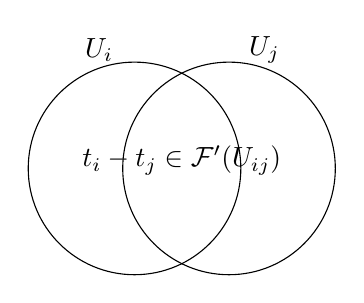
\begin{tikzpicture}
\draw (0,0) circle (1.35);
\draw (1.2,0) circle (1.35);
\node at (-0.45,1.5) {$U_i$};
\node at (1.65,1.5) {$U_j$};
\node at (0.6,0.1) {$t_i-t_j\in\mathcal F'(U_{ij})$};
\end{tikzpicture}
\caption{Two local lifts of the same quotient section differ by a section of the kernel on the overlap.}
\end{figure}
